
% introduction
\begin{frame}[fragile]{Math}{Types of math in latex}
	\footnotesize
    \LaTeX has a monopoly in typesetting math expressions in any context.
    So much that other frameworks like \texttt{MathJax} have integrated
    \LaTeX's code and implementation to render math.     \begin{block}{Inline math}
        This is used to write smaller math expressions within the text.
		Can be activated using.

		\begin{itemize}
		\item \begin{verbatim}\(...\)\end{verbatim}
		\item \begin{verbatim}$...$\end{verbatim}
		\item \begin{verbatim}\begin{math}...\end{math}\end{verbatim}
		\end{itemize}
    \end{block}

    \begin{block}{Math-Mode}

		Used to write larger equation which render on a seperate line.
		Can be activated using.

		\begin{itemize}
		\item \begin{verbatim}\[...\]\end{verbatim}
		\item \begin{verbatim}$$...$$\end{verbatim}
		\item \begin{verbatim}\begin{equation}...\end{equation}\end{verbatim}
		\end{itemize}
    \end{block}

\end{frame}


% some examples
\begin{frame}{Math}{Symbols}
	\footnotesize
	Practically every Math symbol
	or equation that you have ever seen printed on a text book can be
	written in \LaTeX. But you may need some extra packages to render different
	symbols. \vspace{1em}

	\href{https://oeis.org/wiki/List\_of\_LaTeX\_mathematical\_symbols}{Here} is a
	website containing a list of widely used symbols in latex.

	\begin{columns}
		\begin{column}{0.5\textwidth}
			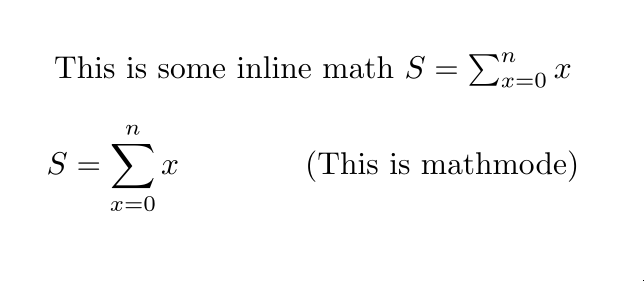
\includegraphics[width=\textwidth]{math1.png}
		\end{column}
		\begin{column}{0.5\textwidth}
			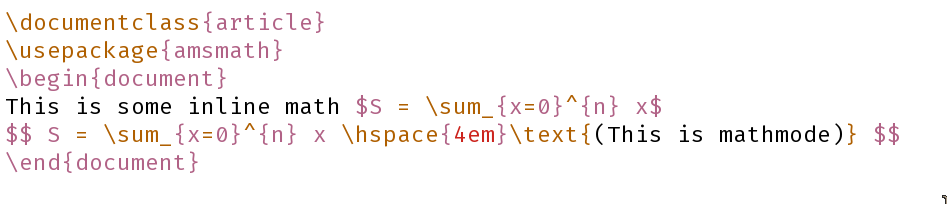
\includegraphics[width=\textwidth]{math1_code.png}
		\end{column}
	\end{columns}

	\begin{columns}
		\begin{column}{0.5\textwidth}
			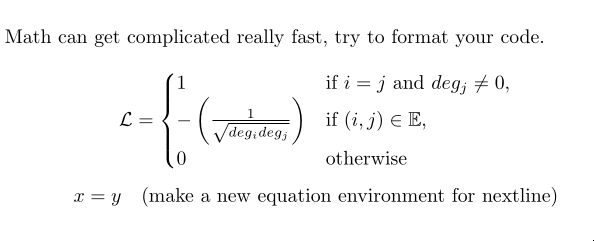
\includegraphics[width=\textwidth]{math2.png}
		\end{column}
		\begin{column}{0.5\textwidth}
			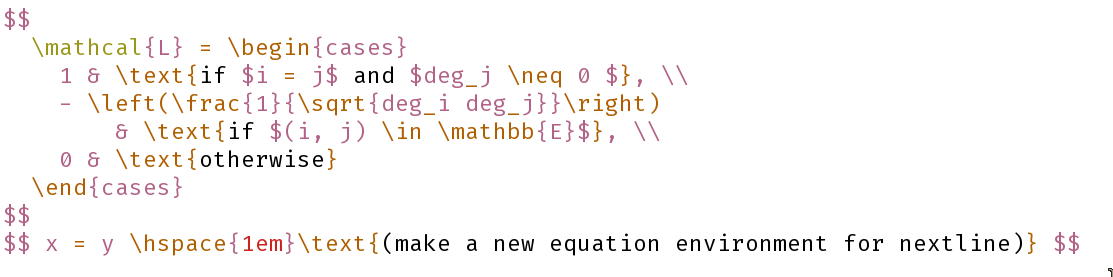
\includegraphics[width=\textwidth]{math2_code.png}
		\end{column}
	\end{columns}

\end{frame}


% task
\begin{frame}{Math}{Task-2}
	Its impossible to go through plethora of features in Math, you learn
	as you come accross stuff.
    Try solving the task-2.
$$ \int_{1}^{x} \sum_{p\leq u}\left\lceil \frac{\log u}{\log p} \right\rceil \log p.du
= \frac{\hbar}{2\pi \iota}\int_{c-\iota \infty}^{c+\iota \infty}
\frac{x^{s+1}}{s(s+1)} \left( - \frac{\partial\zeta '(s)}{\partial\zeta(s)} \right).ds$$
\end{frame}
